\documentclass[sigplan,10pt]{acmart}
\usepackage[utf8]{inputenc}
\usepackage{todonotes}

\copyrightyear{2019}
\acmYear{2019}
\setcopyright{acmlicensed}
\acmConference[PaPoC '20]{7th Workshop on Principles and Practice of Consistency for Distributed Data}{April 27, 2020}{Heraklion, Greece}
\acmBooktitle{7th Workshop on Principles and Practice of Consistency for Distributed Data (PaPoC '20), April 27, 2020, Heraklion, Greece}
\acmDOI{}
\acmPrice{}
\acmISBN{}

\hyphenation{Web-RTC}

\begin{document}
\title{PushPin: Towards Production-Quality  Peer-to-Peer Collaboration}

\author{Peter van Hardenberg}
\email{pvh@inkandswitch.com}
\affiliation{%
  \institution{Ink \& Switch, LLC}
  \city{San Francisco}
  \state{CA}
  \postcode{}
  \country{USA}
}

\author{Martin Kleppmann}
\email{mk428@cl.cam.ac.uk}
\orcid{0000-0001-7252-6958}
\affiliation{%
  \institution{University of Cambridge}
  \streetaddress{15 JJ Thomson Avenue}
  \city{Cambridge}
  \state{}
  \postcode{CB3 0FD}
  \country{United Kingdom}
}

\begin{abstract}
Fully peer-to-peer application software promises many benefits over cloud software, in particular, being able to function indefinitely without requiring servers.
Research on distributed consistency mechanisms such as CRDTs has laid the foundation for P2P data synchronisation and collaboration.
In this paper we report on our experience in taking these technologies beyond research prototypes, and working towards commercial-grade P2P collaboration software.
We identify approaches that work well in our experience, such as the functional reactive programming paradigm, and highlight areas in need of further research, such as the reliability of NAT traversal and usability challenges.
\end{abstract}

\begin{CCSXML}
<ccs2012>
    <concept>
        <concept_id>10003033.10003039.10003051.10003052</concept_id>
        <concept_desc>Networks~Peer-to-peer protocols</concept_desc>
        <concept_significance>500</concept_significance>
    </concept>
    <concept>
        <concept_id>10011007.10010940.10010971.10010972.10010540</concept_id>
        <concept_desc>Software and its engineering~Peer-to-peer architectures</concept_desc>
        <concept_significance>500</concept_significance>
    </concept>
    <concept>
        <concept_id>10003120.10003130.10003233</concept_id>
        <concept_desc>Human-centered computing~Collaborative and social computing systems and tools</concept_desc>
        <concept_significance>500</concept_significance>
    </concept>
    <concept>
        <concept_id>10011007.10010940.10010992.10010993.10010961</concept_id>
        <concept_desc>Software and its engineering~Synchronization</concept_desc>
        <concept_significance>300</concept_significance>
    </concept>
</ccs2012>
\end{CCSXML}

\ccsdesc[500]{Networks~Peer-to-peer protocols}
\ccsdesc[500]{Software and its engineering~Peer-to-peer architectures}
\ccsdesc[500]{Human-centered computing~Collaborative and social computing systems and tools}
\ccsdesc[300]{Software and its engineering~Synchronization}

\keywords{real-time collaboration, CRDTs, peer-to-peer protocols, distributed programming, usability}

\maketitle

\section{Introduction}

In the past, software used to run on one computer and store its data on the local disk.
Now, increasingly, we expect our software and data to be available on multiple devices, with synchronisation across devices belonging to the same user (e.g.\ laptop, smartphone, tablet), and also allowing real-time collaboration between multiple users.

The standard way of implementing such multi-user, multi-device software today is to rely on cloud services that store the authoritative copy of the users' data, and which can be accessed through thin clients such as web browsers and mobile apps.
However, reliance on the cloud comes with problems: services require ongoing maintenance by expensive 24/7 operations teams, and they cease to exist when the organisation backing them terminates their funding.
If a cloud service shuts down, users lose access to all data stored in that service, unless some migration path to an alternative service is provided.
Moreover, cloud-centric software often does not work well offline, and can be slow as the client waits for round-trips to the server in order to load or store data there.

Peer-to-peer application software promises to overcome these problems.
In principle, a P2P system should be able to function indefinitely, without depending on someone paying the server bills to keep a cloud service running.
Storing an authoritative copy of data on the users' devices enables offline work and stronger data ownership~\cite{LocalFirst}, and synchronising updates through a P2P network should allow the same kind of real-time collaboration that we know from cloud software.

While various research prototypes of P2P collaboration software have been developed, we are yet to see any mainstream applications using this approach.
Technologies such as Conflict-free Replicated Data Types (CRDTs)~\cite{Shapiro:2011un} and P2P data replication protocols (see Section~\ref{sec:networking}) provide a good foundation for this type of software, but there is still a big gap between these building blocks and the requirements of software with the features expected by users today.

For example, there are at least half a dozen CRDT algorithms for P2P collaboration on a plain text document~\cite{Kleppmann:2019iu}, and various P2P protocols that can replicate a static file.
However, there is little existing work on how to use these building blocks to implement a rich workspace containing potentially thousands of documents and files of various types, with facilities for organising, searching, and selectively sharing this content with other users.

The PushPin project is investigating if and how we can develop commercial-quality collaboration software with minimal reliance on servers.
Our goal is not to create new algorithms or protocols, but rather to evaluate existing technologies by developing an example P2P application with a mindset of industrial software development best practices and realistic user requirements.
We approach this project with broad interests in exploring programming models, P2P data distribution, reliability, and usability.

In summary, our findings are:
\begin{itemize}
    \item CRDTs provide a reliable, principled foundation for P2P collaboration.
    We found the details of conflict resolution semantics to be surprisingly unimportant, as conflicts seem to occur rarely in practice.
    \item The Functional Reactive Programming (FRP) approach is a good way of creating user interfaces on top of state managed by CRDTs (Section~\ref{sec:data-model-ui}).
    \item P2P protocols are poorly supported by many network routers (Section~\ref{sec:networking}).
    Consequently, the use of servers to forward network traffic is sometimes unavoidable.
    \item The performance of CRDTs and P2P replication implementations becomes problematic as the amount of data grows. The storage and processing overheads of current implementations are substantial.
    \item Significant open problems remain, including around authentication and access control, indexing and search, schema evolution and compatibility, privacy, and the usability of systems where some devices are in sync while others are not.
\end{itemize}

% The prize for delivering a truly peer-to-peer application development system is great.
% centralised cloud-based software has created the expectation of universal access to both canonical versions of software and to users' data from any internet-connected computer at any moment, with full collaborative functionality built in.

%To this end, we must reconsider our relationship with vast centralised databases and explore new methodologies for building software.

% document CRDTs
% functional reactive programming
% browser rendering
% "document oriented programming"

\section{Design Principles}\label{sec:principles}

Before going into the details of the implementation of PushPin we outline the principles we applied to its design and development.

\subsection{Local-first software}

While we want users' data to be accessible on multiple devices, the authoritative copies of this data should reside on the users' local computers, not in the cloud.
If servers are used, these replicas should be considered secondary copies that exist only to facilitate data synchronisation and backup, but they should not be considered authoritative.
In previous work we have coined the term \emph{local-first software} to describe software that adheres to this principle~\cite{LocalFirst}.

With a local-first approach, the software continues working fully if the user's computer is disconnected from the Internet: cross-device synchronisation happens in the background when a network connection is available.
Even if all servers are shut down, the copy of the data on the local disk remains fully functional and under the user's control.
The user can manage this data like any other local files, e.g.\ copying it, backing it up, or converting it into another format.

\subsection{Minimal dependence on servers}

We want the software to continue working indefinitely, without being vulnerable to outages if the organisation running some piece of infrastructure goes out of business.
Thus, in addition to local data storage on each device, the cross-device data synchronisation mechanism should also depend on servers to the least degree possible.

In some environments it is possible to operate entirely without servers, while in other cases a small amount of centralised infrastructure seems to be inevitable with current technologies.
However, if servers are used, we want them to be as simple, generic, and fungible as possible, so that one unavailable server can easily be replaced by another.

\subsection{Conflict-free data synchronisation}

The combination of using local on-device storage, support for offline editing, and synchronisation without servers implies that our application is \emph{intrinsically distributed}.
Each device serves as a replica, and it would not make sense to enforce any kind of single system image semantics across replicas, since that would imply that a device must wait for synchronous coordination with other devices whenever any data is changed.
We cannot rely on consensus algorithms, which must wait for communication with a quorum of replicas.

Rather, we have to accept that each device has its own local view onto the shared data, and that those views may diverge as users update their data.
As devices exchange updates, they converge again by merging their states.
We do this using conflict-free replicated data types (CRDTs)~\cite{Shapiro:2011un}.

\subsection{Mainstream, as far as possible}

In order to explore the \emph{user experience} implications of a peer-to-peer architecture, we wanted to develop not just a rough research prototype, but polished end-user software that is on par with commercial applications available today, with a thoughtful graphical and interaction design.
We also wanted to explore the \emph{developer experience} of peer-to-peer software, to understand how writing software with this architecture could become accessible to mainstream software engineers.
Thus, we wanted to base our work on mainstream languages and platforms as far as possible.

\begin{figure*}
    \centering
    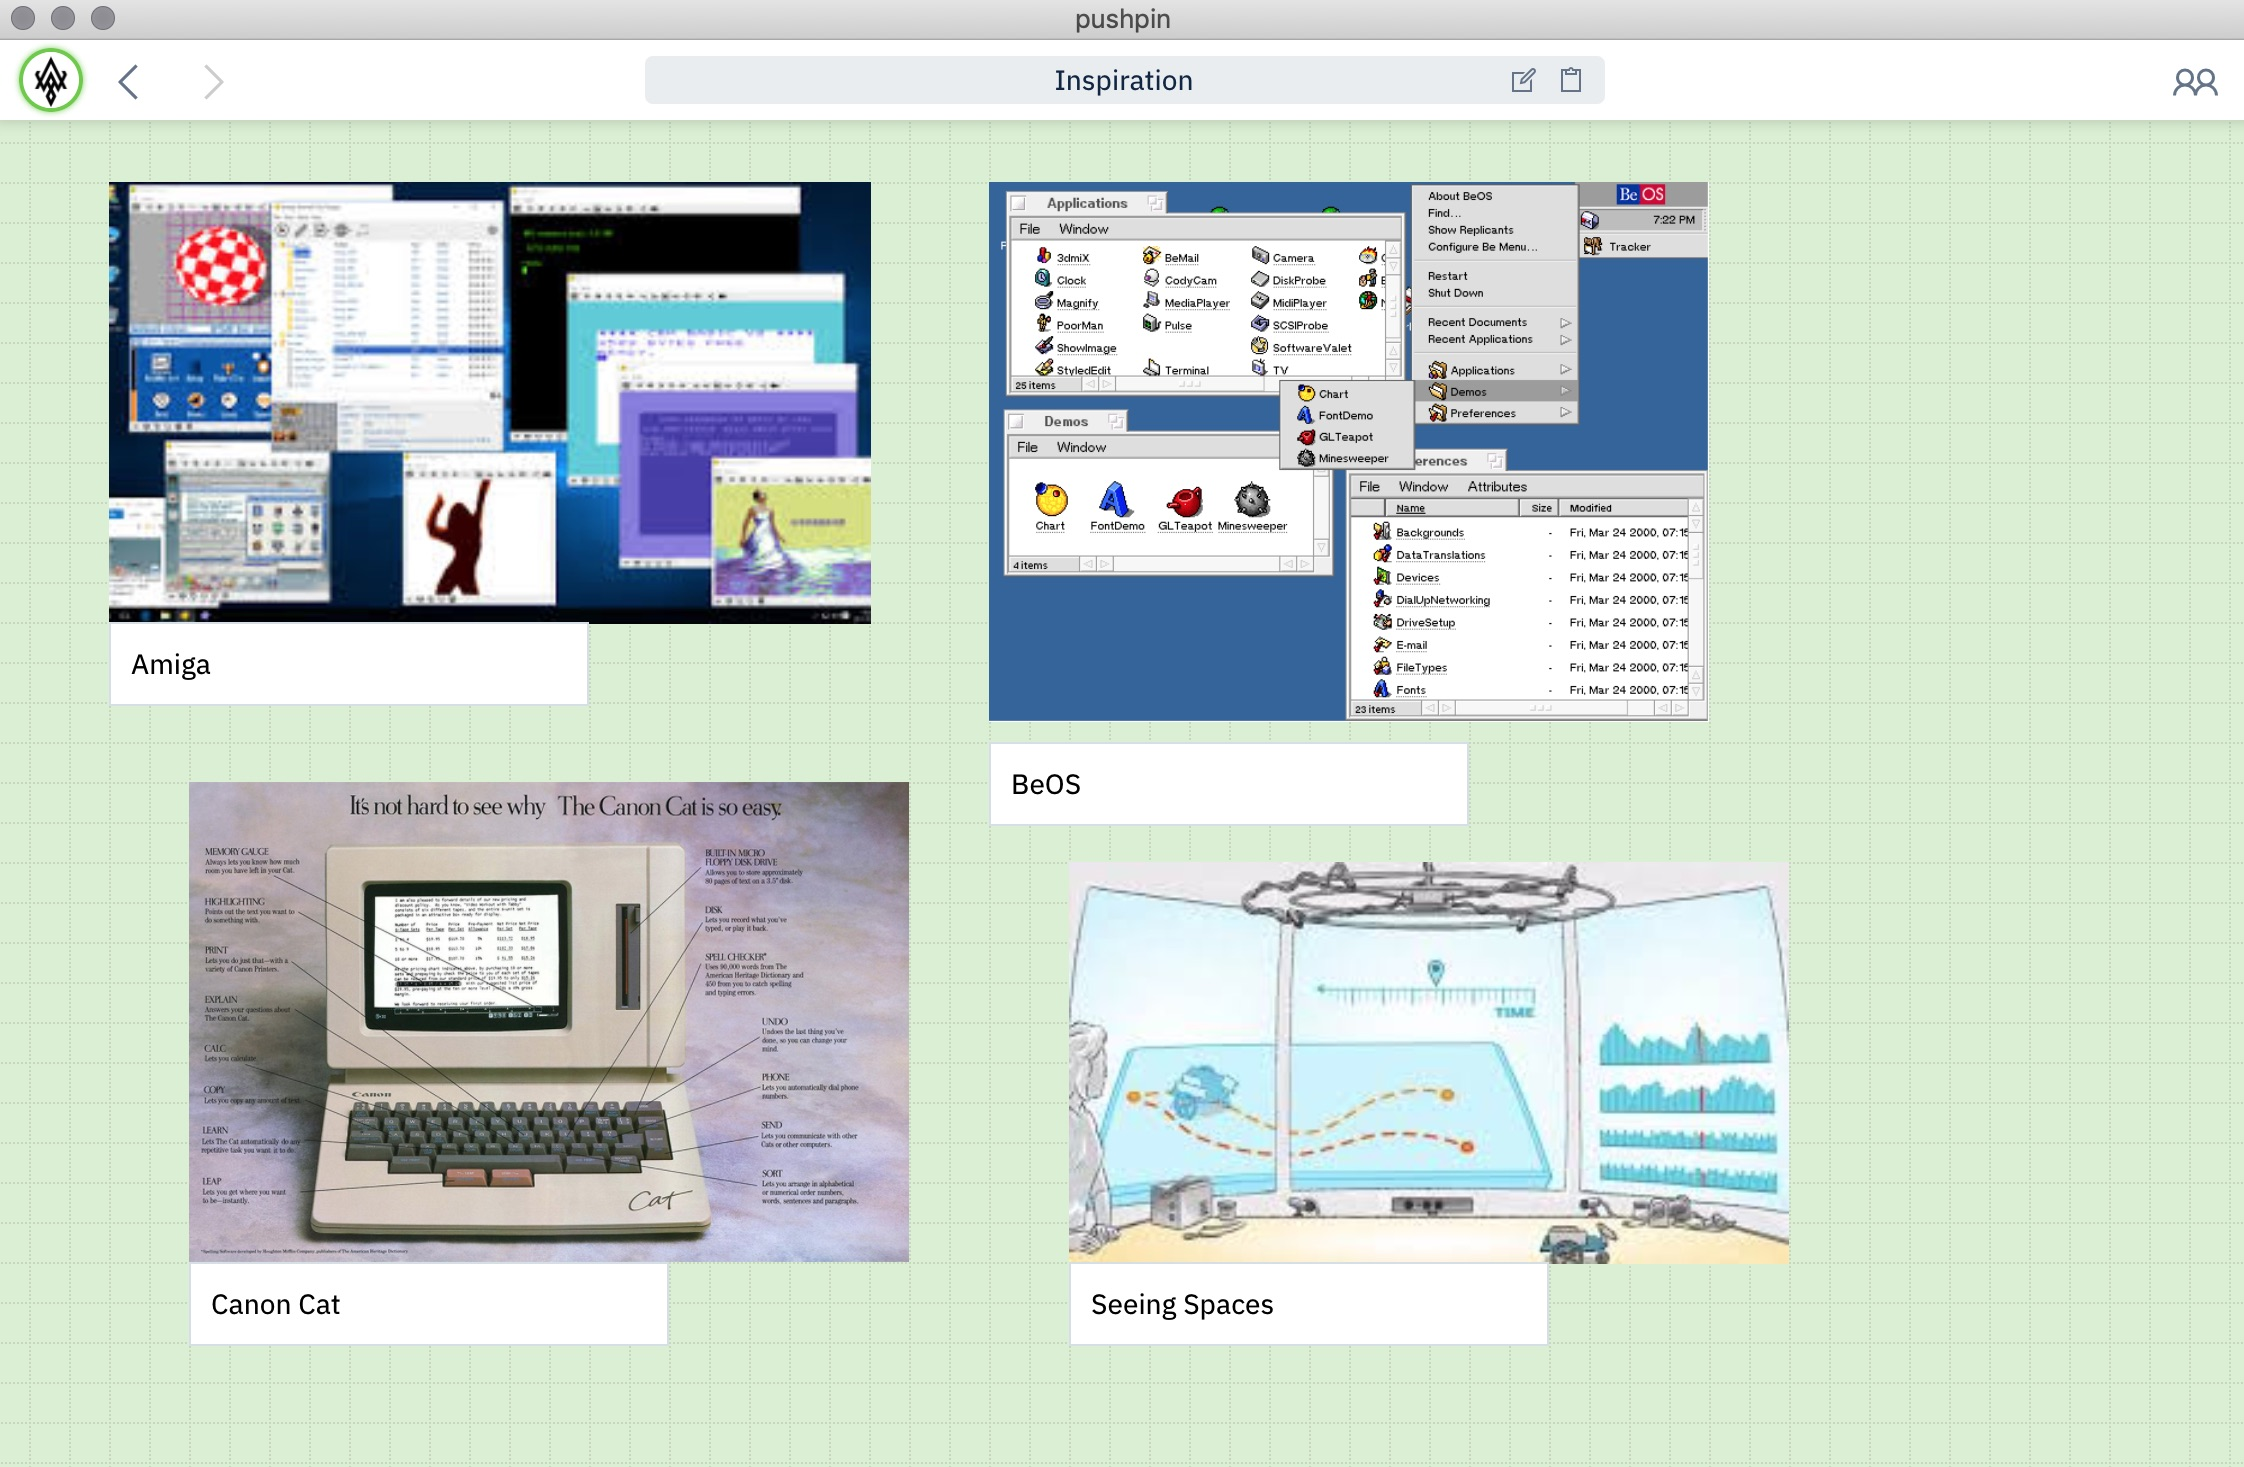
\includegraphics[width=0.7\textwidth]{pushpin.jpg}
    \caption{Screenshot of PushPin. The main user interface consists of cards of various types (text, image, PDF, \dots) that can be freely arranged on a 2D ``board''. Boards can be nested within other boards. The toolbar at the top provides navigation between boards and sharing settings.}
    \label{fig:pushpin}
\end{figure*}

\section{PushPin: A Collaborative Corkboard}\label{sec:pushpin}

The PushPin software~\cite{PushPinSource}, shown in Figure~\ref{fig:pushpin}, allows users to collect media of various types (including text, web pages, images, and PDF files), to archive and organise it.
Media files are visually represented as \emph{cards} on an infinite two-dimensional \emph{board}, where they can be resized and positioned arbitrarily.
One board may be nested within another board, enabling hierarchical organisation and navigation.
This board metaphor is inspired by software such as Miro~\cite{Miro} and Milanote~\cite{Milanote}.

We chose this application because it fits well with the principles articulated in Section~\ref{sec:principles}: the data in this software belongs to the user, and there are essentially no restrictions as to what the user may do with their data.
Unlike some systems (e.g.\ banking or payment systems, auction websites, ride-sharing services, or games), in this application there is no need to enforce any global rules or consensus across users, and there is no need for an authority to decide what actions are allowed.
The only restrictions are access permissions (i.e.\ defining which user may view or modify which pieces of data), but we assume that a user with permission to edit some piece of data may modify it in any way.


\subsection{Building desktop software with Electron}

In recent years there has been considerable innovation in web application technologies, including in web browsers (new features of HTML and CSS), languages (e.g.\ TypeScript), user interface libraries (especially React~\cite{React}), and JavaScript modules for a wide variety of tasks (e.g.\ PDF rendering~\cite{PDFjs}).
In order to take advantage of this lively ecosystem, we decided to implement PushPin using web technologies.

However, web applications running in a browser tab have constraints that make them unsuitable for local-first/P2P use. These constraints fall in two categories:
\begin{description}
\item[Storage.]
By default, browsers do not reliably store data.
Web applications can use localStorage, IndexedDB or Progressive Web App features to store data on disk, but this data is silently deleted when a user chooses to clear cookies in their browser~\cite{LocalStorageCleared}, and browser caches can expire data without notification.
Users have no way of predicting whether their data or the application will be available offline.

Sometimes, manual steps are required: for example, Google Docs requires installing a special browser extension to enable offline support, and it only makes documents available offline when they are specifically selected by the user. Anecdotally, it appears to be common for users to think they had enabled offline usage, only to realise later that their data is unavailable.

\item[Networking.]
For security reasons, web browsers restrict the network communication that application code can perform: client-server requests are restricted to HTTP or WebSocket, and are subject to the same-origin policy \cite{SameOrigin}. Peer-to-peer communication is restricted to WebRTC (see Section~\ref{sec:existing-p2p}).
It is not possible to use arbitrary TCP or UDP networking, which would be required to implement other peer-to-peer protocols.
\end{description}

We avoid these limitations by building on Electron~\cite{Electron}.
Electron runs a JavaScript web application in a dedicated Chromium-based browser runtime, packaged as a downloadable and locally installed executable containing all of the required code.
Once installed, the user can be sure that the application is available offline.

Electron also makes Node.js APIs available to application code, which enables full access to the local filesystem, and socket APIs allowing arbitrary TCP and UDP networking.
Thus, Electron allows software engineers with web development skills to write cross-platform desktop software for macOS, Windows, and Linux.

\begin{figure*}
\begin{verbatim}
{
  "title": "Inspiration",
  "authors": [
    "hypermerge:/BvRmN2rU7pQBginzw9KqTXcUmtyYC5aCLiZZ314Ga8Vt?contentType=contact",
    "hypermerge:/6YTvUkNePGkPJH3fHaCoJfJdVdKbi6qjDKgp27u3SChG?contentType=contact"
  ],
  "cards": [
    { "x": 0, "y": 0, "w": 577, "h": 484,
      "url": "hypermerge:/4uhU1SDgy56cAo3dQH5tqSrrTAZnQSQKkEUPzNUXSvcV?contentType=image" },
    { "x": 0, "y": 486, "w": 577, "h": 95,
      "url": "hypermerge:/HHmxeCceWD1ZBrXKeHPv7k7umVW2ncsWyVrUiV3cmMYP?contentType=text" },
    { "x": 612, "y": 84, "w": 370, "h": 862,
      "url": "hypermerge:/E6qRRVUsbRcjddCV98TLyyRhPsVNgyiUXAdPsLyKM3mn?contentType=todo-list" }
  ]
}
\end{verbatim}
\caption{JSON document representing a PushPin board with three cards on it.}
\label{fig:board-json}
\end{figure*}


\subsection{Automerge Documents}\label{sec:documents}

All application state in PushPin is managed by Automerge~\cite{Automerge:2018,Automerge}, a JavaScript CRDT library that provides a JSON data model~\cite{Kleppmann:2017ca}.
Automerge defines a format in which data updates can be written to local disk and replicated to instances of PushPin on other devices.
Network communication is provided by a separate layer called Hypermerge, which we discuss in Section~\ref{sec:networking}.

An Automerge document is the unit of replication and sharing in PushPin: that is, a user can access either all or none of a document.
We want a PushPin user to be able to share their content with other users at a fine-grained level: e.g.\ one card at a time, or one board at a time.
For this reason, we represent each card and each board as a separate document.

For example, Figure~\ref{fig:board-json} shows the JSON representation of a board.
It contains a \texttt{title} (rendered in the toolbar in Figure~\ref{fig:pushpin}), a list of users who have contributed to the board, and a list of cards on the board.
Each card has \texttt{x} and \texttt{y} attributes recording its position, \texttt{w} and \texttt{h} attributes for width and height, and a \texttt{url} linking to its content (in a separate document).

Automerge allows state to be concurrently updated on different devices, and it ensures that replicas converge to the same state as they communicate.
For example, if a user drags a card to a new position, this state change is modelled by updating the \texttt{x} and \texttt{y} attributes of that card, while the rest of the document remains unchanged.
If another user concurrently creates a new card on another device, it is inserted into the list of cards.
The CRDT tracks that change and records it as an Automerge operation for replication.
The concurrent updates (changing the position of one card and adding another card) are merged cleanly on each replica.

\subsection{URLs and Linking}\label{sec:urls}

Each document is identified by a unique \texttt{hypermerge} URL of the form shown in Figure~\ref{fig:board-json}.
Given a URL, a PushPin instance can obtain the corresponding document content through a process described in Section~\ref{sec:peer-discovery}.
By including one document's URL in the content of another document, we form a graph of links, similar to the web.

The same URL can be referenced from multiple places, allowing e.g.\ the same card to be embedded on multiple boards.
URLs can also be shared with another user by sending them through any communication channel, such as email.
When a PushPin instance loads a document containing a \texttt{hypermerge} URL, it eagerly resolves and downloads the content belonging to that URL.
Thus, any transitively reachable documents are automatically added to PushPin's local document storage on that device, making them available offline.

Each URL also includes a \texttt{contentType} parameter, which indicates how that document should be rendered in the user interface.
This parameter is part of the URL, not the document content, because the same document content may be rendered differently in different contexts.
For example, PushPin could be extended to support flashcards for language learning.
In one context, the document containing the database of flashcards could be rendered as a list of entries, while in another context it might be rendered as a quiz interface, presenting one side of one card at a time.

\begin{figure*}
\centering
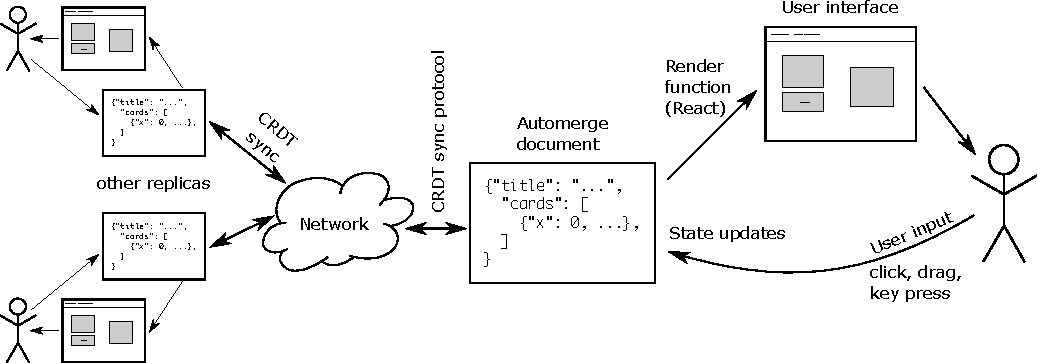
\includegraphics{document-frp.pdf}
\caption{The data flow of Document Functional Reactive Programming (DFRP).}
\label{fig:document-frp}
\end{figure*}

\section{Creating User Interfaces for CRDTs}\label{sec:data-model-ui}

In traditional, server-centric web applications, synchronisation between client-side and server-side state is usually performed in an ad-hoc way, with user actions translating into HTTP requests that perform API calls on a server.
In contrast, CRDTs provide us with a principled way of managing and reasoning about the state of multiple replicas: each replica can optimistically update its local state, and a synchronisation protocol running in the background ensures that those replicas eventually converge~\cite{Saito:2005jw}.

However, the convergence we have discussed so far is at the level of Automerge documents, such as the JSON shown in Figure~\ref{fig:board-json}.
In this section we will expand the discussion to include the state of the user interface.

\subsection{Functional Reactive Programming (FRP)}

For PushPin we wanted a similarly principled approach to developing user interfaces, which would allow the state of the CRDT and the state of the user interface to be kept in sync in a way that is robust and easy to reason about.

We solved this problem using the Functional Reactive Programming (FRP) approach~\cite{Czaplicki:2013ig}, which has been gaining popularity in JavaScript web applications, especially due to its implementation in Facebook's React library~\cite{React}.

FRP works by defining a deterministic \emph{render} function that takes the current state of an application and returns a description of a user interface that displays this state.
Whenever the user performs an action, rather than updating the user interface directly, the \emph{state} is updated to reflect that action.
The updated state is then passed to the render function in order to determine the updated user interface.
In practice, performance is improved by detecting which parts of the state are unchanged, and rendering and updating only those parts that have changed.
However, the conceptual simplicity remains: the render function cleanly translates between application state and user interface state.

\subsection{Document FRP (DFRP)}

In the usual implementation of FRP, the application state (the input to the render function) is simply an in-memory object.
In PushPin, we generalise this approach by making an Automerge document the input to the render function.
We call this approach \emph{Document FRP} (DFRP).

Figure~\ref{fig:document-frp} illustrates the DFRP data flow.
An Automerge document may be newly created, or loaded from local disk, or fetched over the network.
Regardless of its origin, the document can be displayed by passing it to the deterministic render function.

The resulting user interface has attached event handlers that detect user input, such as mouse clicks or keyboard input.
When any such events occur, the Automerge document is updated to reflect the user input, and the render function is called again to refresh the user interface.
This local interaction can be performed regardless of whether the user is currently connected to the Internet.

Likewise, whenever the network synchronisation protocol running in the background receives an update from another replica, Automerge applies this update to the CRDT state.
We then again call the render function with this updated state, which refreshes the user interface accordingly.
Thus, the user interface logic makes no distinction between a local user's updates and remote updates received over the network: both simply result in a call to the render function.

In applications written in the DFRP style, the developer never needs to worry about API calls to a server backend, or the fact that they may fail.
Instead, all communication is via shared CRDT state that can be updated by any collaborator at any time.
This means DFRP software can actually be \emph{simpler} to develop than traditional web applications, even though it is also more powerful.

% challenges: getting into weird states, write permissions

\subsection{Ephemeral Versus Persistent State}

In our earliest experiments we put all application state into the CRDT. This quickly proved to be problematic: for some types of state, such as unsubmitted text in HTML textboxes or cursor positions, each PushPin instance should have its own state~--- making all replicas converge to the same state is undesirable in these cases.

Also, some fast-changing data, like cursor position or timers for performing animations, can swamp the CRDT with low-value information; there is no reason to persist such updates.
We therefore extended the application state so that it consists of two parts: persistent state that is replicated, and ephemeral state that exists only locally.

However, we may want to share some of this ephemeral data with peers that are currently online: it can be helpful to see whether other users are viewing the same document as you, where their cursor is located, or which items they have selected. It might be interesting to see another user's current position in a podcast or video, or a hint that shows they are currently typing into a chat textbox but have not yet submitted.

For ephemeral updates PushPin uses an additional messaging channel, adjacent to the CRDT, which ties arbitrary messages to a device and user context. The current implementation is rudimentary: ephemeral data is not associated with a particular CRDT state, and is distributed only over live connections, so it will not function as expected in complex network topologies or at large scale. Nevertheless, it has allowed us to add important contextual awareness to the user experience of PushPin. In distributed applications it is particularly important to communicate the feeling of presence when other users are online or collaborating.

% Cut this because we haven't yet explained the degrees of offline/online-ness at this point in the article, making this statement confusing:
%
% because unlike in a centralized system there are many ways to be both online or off

\subsection{Supporting Multiple Documents}

Sections~\ref{sec:documents} and~\ref{sec:urls} explained how PushPin breaks down all of its data into fine-grained documents.
This decomposition of state is also beneficial for user interface development, because rendering can be done at the document level.

For example, we can have a function that renders a text card, and that renderer can be invoked wherever a text card appears.
This makes the user interface components more easily reusable and composable.
It is also easy to extend the application with new renderers, allowing users to have boards containing a mixture of predefined card types and custom card types they have defined themselves.

Moreover, we can have multiple renderers that are able to render the same document in different ways.
For example, in the user interface shown in Figure~\ref{fig:pushpin}, the board is actually being rendered twice: firstly as a 2D space representation containing the cards, and secondly the toolbar displaying the title of the board and its authors.

\subsection{High-Performance User Interfaces}

In order for user interactions with software to feel smooth, the user interface should render at a rate of 60 frames per second.
We therefore aim to never block the user interface thread for more than 16 milliseconds.

However, some CRDT computations, cryptographic operations, and similar tasks can easily exceed this time budget.
We address this problem by performing as much as possible of this work on a background thread.
Automerge is split into a frontend that runs on the user interface thread, and a backend that runs on the background thread, with an asynchronous message-passing protocol between the two.

Moreover, Automerge allows local user input to be applied immediately to the document state in the frontend, without waiting for any communication with the backend.
This allows the application to minimise the time between user input (such as pressing a key) and the corresponding update appearing on the screen.
Automerge transparently handles the fact that local user input in the frontend can happen concurrently with the backend processing remote operations.
We have not seen any other CRDT implementation that provides this feature.


\section{Peer-to-peer Networking for Collaboration}\label{sec:networking}

Every networked application relies on three core facilities provided by the networking stack: discovering the network address to connect to, establishing a connection, and securing the confidentiality and integrity of the data transfer.

In a traditional web application, discovery is provided by DNS, connection by TCP, and security by SSL/TLS.
However, these technologies are designed for centralised infrastructure, and they are not a good fit with our goal of being resilient to infrastructure failures:
\begin{itemize}
    \item DNS records disappear if the domain name owner stops paying the required registration fees, or stops running the authoritative nameserver.
    \item TCP requires a server with a publicly routeable IP address; it cannot connect directly to most end-user devices as they are behind NAT (see Section~\ref{sec:nat-traversal}).
    \item SSL/TLS certificates are tied to domain names, which incur registration fees.
\end{itemize}

The peer-to-peer technologies we explored in PushPin attempt to overcome the need for centralised infrastructure.

\subsection{Existing Peer-to-Peer Technologies}\label{sec:existing-p2p}

We considered several P2P networking stacks for PushPin:
\begin{description}
\item[WebRTC] is a peer-to-peer protocol built into modern web browsers.
It is primarily designed for audio and video calls, but it can also carry application data.
WebRTC does not provide a peer discovery mechanism; typically, applications rely on a server to help peers discover each others' IP addresses (this process is called \emph{signaling}).
\item[BitTorrent] is widely used for file sharing.
It provides a distributed hash table (DHT) for peer discovery, and uses the uTP protocol to establish connections between peers.
However, it is designed for static files, and is not suitable for data that is constantly changing, like in collaboration software.
\item[IPFS] aims to provide decentralised storage through a networking stack called \emph{libp2p}.
Like BitTorrent, it is mostly focused on replicating static files; it provides limited support for changing data through its IPNS and PubSub modules, but these features are immature at the time of writing.
\item[Dat] \cite{HowDatWorks,Ogden:2018ur} is a peer-to-peer data sharing platform.
For peer discovery it uses a centralised DNS service hosted by a nonprofit foundation (a DHT is under development), and it uses BitTorrent's uTP protocol to establish connections.
\end{description}

For PushPin we decided to build upon the \emph{hypercore} protocol and implementation from the Dat project, since its focus on replicating mutable data makes it the best fit for our needs.
Our integration of Hypercore with Automerge is called \emph{Hypermerge}~\cite{Hypermerge}.

A hypercore is an append-only log that is authenticated with a public key; only the owner of the corresponding private key can modify the log, but many peers can store replicas of the log.
We map each Automerge document to a set of hypercores, with one hypercore per device that has edited the document.

\subsection{Peer Discovery}\label{sec:peer-discovery}

The Dat protocol allows the replicas of a hypercore to be discovered based on a hash of its public key~\cite{HowDatWorks}.
We construct the URL for a document by encoding this public key.
Thus, the URL is a stable identifier for the document, even as its content changes, and knowledge of the URL allows a peer to obtain a copy of the document via the peer discovery mechanism.

When peers are on the same LAN (wired or wireless network), they attempt to discover one another using mDNS, a variation on DNS that broadcasts DNS-like service advertisements or discovery requests to a well known multicast IP address.
If successful, the peers can connect directly via TCP and begin exchanging data.
This mode of discovery is appealing since it depends only on the local network: communication between peers does not flow via the Internet, and it does not depend on any centralised infrastructure.

When peers are not on the same LAN, the Dat protocol uses a centralised DNS server for peer discovery.
This approach is not fully peer-to-peer, but at present this seems to be a necessary compromise to make.
Since the DNS server only provides peer discovery, and does not handle any data transfer traffic, it is quite cheap to run.

\subsection{NAT Traversal}\label{sec:nat-traversal}

Due to a shortage of IPv4 addresses, most personal computing devices do not have a globally reachable IP address, but rather a local address in a reserved space (e.g.\ 192.168.x.x or 10.x.x.x).
When such a device wishes to establish a connection to another, the local router records the destination of outbound traffic and routes responses back to the originating local client.
This process is called Network Address Translation (NAT).

A device behind a NAT router can make outbound connections, but it cannot receive inbound TCP connections from outside of the NAT.
An exception: in home environments, where the user has control over their own router, the UPnP standard allows devices to reserve particular ports on the router's public IP address as the destination for inbound connections.
However, mobile devices often use networks with NAT on which UPnP is not available, such as a coffee shop WiFi, a corporate office network, or a cellular data network.

In these cases, the most viable solution is known as ``hole punching'' or NAT traversal \cite{RFC5389}.
This process requires the temporary intervention of a third host to introduce the two peers, and both peers sending UDP packets to each other, allowing a connection to be established.
NAT traversal is performed by BitTorrent's uTP\cite{BEP29} protocol, and by the STUN protocol in WebRTC \cite{RFC5389}.

However, there are situations in which neither the LAN discovery approach nor NAT traversal works.
For example, some coffee-shop WiFi and some corporate networks are set up in a ``guest network'' mode, which prevents all local connections between devices on the network (intended as a security measure to prevent inadvertent sharing of data with other users on a public network).
Without local traffic, we attempt to fall back on NAT traversal; however, this approach also fails, since many routers in their default configuration refuse to create NAT traversing routes that originate and terminate within the same network.

In this case, establishing a direct connection between the peers seems to be impossible, and the only remaining option is to use a server with a public IP address to proxy the communication between the peers, e.g.\ using the TURN protocol~\cite{RFC5766}.
In the case of PushPin, users can either run their own publicly addressable network hosts or take advantage of a TURN server provided by the community.

\subsection{Storage Peers}

A limitation of any peer-to-peer system is that two peers can only communicate while they are both online.
However, mobile devices are often offline, potentially making it difficult to find an opportunity to synchronise.
For example, if your colleague has shared the URL of a PushPin board with you, it would be annoying if you could not access that board because the only copy of the board resides on your colleague's laptop, and that laptop's lid is currently closed.

We can overcome this limitation by introducing \emph{storage peers}, which replicate all the data belonging to a particular user or set of users.
A storage peer runs the same replication code as PushPin, recursively following any Hypermerge URLs, but as a simple Unix daemon without any visual user interface.
The storage peer can be deployed on a server or other computer that is always online, allowing other devices to sync with the storage peer at any time.
Storage peers also provide a form of backup.

Unlike a traditional server, a storage peer can be reached through NAT traversal, so it does not need a public IP address: for example, it could be a device on the user's home internet connection.
Since it only stores the data for a small number of users, it does not need to be a powerful machine.
We have experimented with using a Raspberry Pi as storage peer, writing data to an SD card.

An interesting detail of the PushPin storage peer is that its user interface is not a web interface, nor a command line interface, but an Automerge document.
When it starts up, the storage peer prints a URL that users can load from PushPin on another computer.
Users then interact with their storage peer by making edits to this adminstration document within PushPin.
The storage peer daemon monitors that document for changes and takes actions based on what it finds.

\subsection{Data Confidentiality and Integrity}

Some peer-to-peer systems, such as BitTorrent and IPFS, use a content-addressable storage approach to data integrity: every file is identified by the hash of its contents, and the recipient can check the integrity of the file by comparing its actual hash to the expected hash.
(In fact, BitTorrent uses Merkle trees \cite{Merkle:1987} to allow efficient incremental validation of data during its download.)
However, this approach is not suitable for collaboration software, where the the hash would frequently change as data is modified.
Instead, Dat relies on digital signatures to ensure that nobody can make undetected alterations to the data without knowing the private key.

The Dat protocol encrypts the communication between peers, using the URL of the document as a shared secret to establish the encryption key~\cite{HowDatWorks}.
Thus, the URL acts as a bearer token (or capability) that grants read access to the document to anyone who knows it.

A downside of this approach is that there is no real way of revoking a user's access to a document.
It is possible to generate a new URL and copy the document content, but this breaks any links to that document.
We are interested in stronger access control and end-to-end encryption protocols for collaboration software that allow key rotation and revocation~\cite{Kleppmann:2018tk}, but we have left this issue out of scope in the PushPin project.

The peer discovery protocol uses hashes of URLs, not the URLs themselves, so that anyone observing the peer discovery traffic (such as the DNS server, or other devices on the local network when using mDNS) does not gain the ability to read the document.

\subsection{Scalability of Peer Discovery}

% (It should be noted that in practice today, the BitTorrent DHT has proven itself operationally resilient but other implementations such as IPFS have struggled to remain useful during flooding attacks.)

On a local network, a Dat peer broadcasts all the hashes of URLs for data it holds, and all the hashes it requests.
This approach is suitable when the number of URLs is small, but it breaks down as collections expand.
Since PushPin uses a separate URL for each card, a user quickly accumulates many hundreds or thousands of document URLs.
In our testing we found that we could fairly reliably crash the consumer-grade WiFi routers found in short-term rentals with half a dozen researchers sharing their collections.

% TODO: diagram of append-only logs, discovery keys, maybe broadcasting?

The Secure Scuttlebutt~\cite{Tarr:2019ba} project avoids this problem by placing all of a user's activity into a single log, which it then merges with all of that user's peers and their peers out for several degrees of social connection. This trades one problem for another: by merging all of a user's data (and their peers' data) into one feed, there is no way to selectively synchronise that user. A peer either downloads all, or none.

Fortunately, we have observed that users tend to collaborate on more than one document with the same collaborator.
Thus, when searching for peers that have a copy of a new document, it is likely that this document of interest can be found in the repository of a peer you are already connected to.
We can significantly reduce the amount of discovery network traffic by first querying existing peers, and only performing a global DHT lookup if this fails.
Perhaps these peers could also forward queries on our behalf, recreating a DHT-like network.
This is an area for future work.

\subsection{Metadata Privacy}

A downside of peer-to-peer protocols is that the peer discovery mechanisms leak information about users to other nodes on the network.
Although the content of documents is only available to peers who know their URLs, the discovery keys (hashes of URLs) are widely broadcast, allowing a user's device to be identified by the pattern of discovery keys it shares.
With this information, an attacker can monitor a user's IP address over time, and thus track their approximate physical location.

A number of defences could reduce this tracking potential (e.g.\ automatic rotation of discovery keys, or some form of interactive proof exchange through a third party prior to exposing IP addresses), but this remains an area of active concern and research.

\section{Conclusions}

Let us begin by reiterating our objectives. We define success as delivering software which is fast, reliable, and useful. By that we mean specifically that the software should:
\begin{itemize}
    \item respond on the next frame to all input
    \item allow local progress at all times
    \item allow collaboration in all network conditions
    \item should not rely on any singleton or centralised services
\end{itemize}

We believe that distributing data stored in the Automerge CRDT over a peer-to-peer system based on Dat, interacting with the data through a React FRP rendering engine and delivering it to clients as an Electron application meets these goals.

\subsection{CRDT / Application Model}

In more detail, associating an Automerge CRDT to an HTML user interfaces via  the FRP programming model reduces complexity for authors of distributed systems. This is because it funnels local and remote changes through a consistent process and eliminates ad-hoc calls to APIs. All CRDT changes can be distributed either live or asynchronously, providing real-time collaboration by default.

Complex application states can be built up by rendering several related documents (directories, text notes, user profiles) each with their own context-specific rendering function for a particular CRDT. The URLs to describe these CRDTs should be self-validating and remain stable during changes. (Content hashing is not effective.)

\subsection{Networking}

Peer-to-peer networking has three stages: content discovery, connection, and synchronisation. The most promising techniques for discovery are based on the distributed hash tables pioneered by BitTorrent, supplemented by mDNS locally. Connection is complicated by the widespread assumption of client-server architectures and widespread NAT routing, and connectivity in public environments like cafes and corporate offices can be particularly challenging.  The state of the art for NAT traversal in public environment is "hole punching", PushPin uses UTP to mitigate this, a NAT-traversing protocol inherited from BitTorrent, but it is imperfect. As with BitTorrent, by replicating self-validating data, the system avoids many concerns about trusting data origin.


\subsection{Future work}
\begin{itemize}
    \item Migrating data between versions and preventing invalid document states remains a concerning problem
    \item Establishing direct peer-to-peer connectivity is problematic in several important environments
    \item Distributed Hash Table side channels are a concerning source of privacy leaks
    \item The PushPin implementation assumes all writes are accepted, an obvious area for additional research \& development
    \item New and old networking stacks have promise to improve connectivity, including BLE, WiFiDirect, and ultrasonic modems
    \item PushPin currently leaves almost all data un-encrypted, requiring trust in any peer that stores your data
    \item The need for rotation of public keys for data is a known and unexplored issue
    \item Some form of efficient document query or index documents are needed -- displaying a list of titles for documents requires fully loading all searchable documents
\end{itemize}

\begin{acks}
Thank you to Roshan Choxi, Ignatius Gilfedder, Mark McGranaghan, Jeff Peterson, and Matt Tognetti, who contributed to the development of PushPin.
The project was produced under the auspices of the Ink \& Switch research lab (\url{https://www.inkandswitch.com/}).
Martin Kleppmann is supported by a Leverhulme Trust Early Career Fellowship and by the Isaac Newton Trust.
\end{acks}

\bibliographystyle{ACM-Reference-Format}
\bibliography{references}{}
\end{document}
